\section{The Journal-Relative Web}
\label{sec:journal-web}

This section combines the state, history, and interpretation layers of \cref{sec:integrity-state,sec:history-entanglement,sec:self-encoding} into a Web in which each \glslink{journal}{journal} serves as its own point of reference. It describes how resources are named, accessed across organizational boundaries, and governed by local rules.

\subsection{A Web of Resources}

The conventional Web organizes interaction around sites, origins, URLs, \glslink{resource}{resources}, representations, links, and clients~\cite{Jacobs2004webarch,BernersLee2005uri}, and the \glslink{synchronic-web}{Synchronic Web} gives each term a historical counterpart. A journal resembles a site with its own administration and evolving state. Its root supplies an origin for interpretation, a \glslink{path}{path} identifies a resource from that root, and a committed \glslink{head}{head} selects the historical view in which resolution occurs. The returned representation may be bytes, an expression, a partial proof, or a \glslink{self-encoding}{self-encoding} \glslink{object}{object}. A path such as \texttt{(*state* components c17 inspection)} lists segments from the journal root, like a filesystem path, where \texttt{*state*} names the application namespace and the remaining segments select nested resources. Such a path gives a resource continuity across versions, while a \glslink{digest}{digest} identifies the exact state found there at one head. A client can therefore request the current resource, resolve the same path at an earlier \glslink{index}{index}, or cite one particular representation by digest. Paths cross semantic as well as structural boundaries, and one segment may enter a tree, another an object, and another a remote history retained beneath a \glslink{bridge}{bridge} (\cref{sec:network-history}). Each object interprets its documented portion, and end-to-end evidence is preserved across every boundary. Because historical states remain addressable, ordinary links embedded in representations can cite a persistent version rather than only a moving current resource. Relative references remain ordinary URI references interpreted by the client against the selected resource~\cite{Rivest1996sdsi,Mazieres1998path}.

Every journal thus induces a distinct coordinate system over local and remote state. A bridge segment encodes the relationship through which remote state became reachable, a historical index selects the committed viewpoint, and content-derived identifiers name exact representations~\cite{Haber1997secure,Kuhn2014trusty,Zhang2014named}. The practical consequence is that a prior state joins the same address space as the current one. Partial evidence can travel as its representation, and clients can distinguish unknown structure, empty structure, unavailable data, policy denial, and unreachable endpoints.\footnote{A committed read can return the absolute local and per-hop indexes selected by that same operation through optional index metadata, so the client can turn a current-head selection into a fixed historical reference.}

\subsection{Access Across the Web}
\label{sec:access-paths}

A path names a resource relative to the journal that resolves it, and the same form extends across bridges. The canonical public form is one flat journal-relative path: an index at the origin journal, then each directional bridge alias followed by a destination index, then a namespace and a local path interpreted at the destination journal. Thus \texttt{(20 carol 15 bob -3 *state* docs report)} selects a historical index at every journal, and negative indexes count back from the latest, so \texttt{-1} selects the current head and \texttt{-3} the head two steps earlier. The alias-and-index prefix is the path's \glslink{route}{\emph{route}}, the sequence of journal-to-journal bridge hops that reaches the destination. Aliases are receiver-local names with no global meaning, and indexes may be omitted when current. Live \texttt{put!}, \texttt{use!}, and \texttt{copy!} follow the current committed object at each hop. \texttt{retrieve} instead combines that current route for \glslink{authentication}{authentication} and endpoint context with independently selected historical indexes for content. Returned evidence may fill a \glslink{stump}{stump} only when its digest remains fixed. A route never advances an embedded remote head to a newer one; each hop uses the exact state committed beneath its parent, which is what allows every hop of the route to be verified against evidence the origin already holds.

\Cref{fig:federated-invocation} shows the exact-object handshake and direct invocation at the destination:

\begin{itemize}
  \item \textbf{Exact forward route.} From A's selected committed head, each hop follows the nested journal object already stored there, through intermediate journal B, until A reaches the exact C object containing C's interface signing key, endpoint, and index/digest context.
  \item \textbf{Receiver-relative return.} C returns a partial object at that same historical C head containing C's reverse route to A's interface key. A requires its index, digest, and reverse sequence to agree with the C object already committed beneath A's forward route~\cite{dinh2025identity}.
  \item \textbf{Direct application call.} A signs and sends the C object with the resource invocation directly to the committed canonical endpoint.\footnote{Intended production deployments use HTTPS.} C matches the raw supplied-object digest against its own history before evaluation, reconstructs the bridge \glslink{principal}{principal} that names A, checks the signature against the key reached by the reverse route, and authorizes the request locally. Intermediaries see public route/control metadata, while the private function, path, arguments, and value travel only on the final connection.
  \item \textbf{Result and retention.} Live invocation results receive only operational assurance, from the direct connection to the committed endpoint. \texttt{retrieve} additionally returns proof that A verifies against the selected historical C object. A may then retain that proof locally with a separate \texttt{pin!} over the full origin-relative historical path.
\end{itemize}

Invocations normally reach the attributed source in this way, but when that source is unavailable or should not be contacted, a client can instead select a retained responder. The responder interprets the requested history locally and serves only permanently retained evidence under its usual \glslink{authorization}{authorization}, resolving current-head selections against what it actually holds and reporting which indexes it retains. The origin anchors the proof to the responder's exact authenticated object and independently derives those selections before verifying the content. \Cref{tab:resource-operations} groups the public resource operations by architectural purpose.


\begin{figure}[htbp]
  \centering
  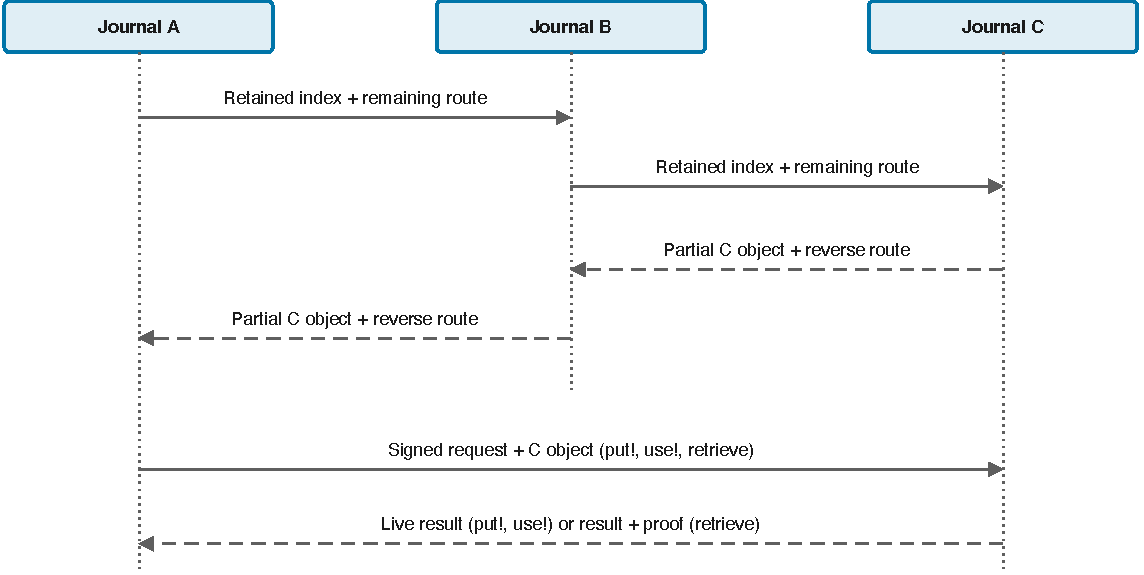
\includegraphics[scale=0.851]{figures/federated-invocation-sequence.pdf}
  \caption{Exact-Object Route and Invocation}
  \label{fig:federated-invocation}
\end{figure}

\begin{table}[htbp]
  \centering
  \small
  \begin{tabularx}{\textwidth}{@{}P{0.25\textwidth}P{0.285\textwidth}X@{}}
\toprule
\textbf{Purpose} & \textbf{Operations} & \textbf{Architectural Boundary} \\
\midrule
Store and copy & \texttt{put!}, \texttt{put-batch!}, \texttt{copy!}, \texttt{copy-batch!} & Change staged state, including deletion. Copy reads sources from one pre-mutation snapshot. \\
Exercise current objects & \texttt{use!}, \texttt{use-batch!} & Invoke objects, persisting successors atomically or discarding them in read-only mode. \\
Compose live operations & \texttt{run!} & Execute a stored program through a caller-bound journal capability. Nested calls keep their own authorization and mutation boundaries; the whole program is not atomic. \\
Retrieve historical evidence & \texttt{retrieve}, \texttt{retrieve-batch} & Read selected committed state or compute an object result from that state, verifying returned evidence without persisting successors. \\
Retain or release evidence & \texttt{pin!}, \texttt{pin-batch!}, \texttt{unpin!}, \texttt{unpin-batch!}, \texttt{prune!}, \texttt{prune-batch!}, \texttt{truncate!} & Change local retention without changing the selected historical commitments; authority and protected-path constraints remain local. Administrator-only truncation releases history through an index while preserving chain identity and numbering. \\
\bottomrule
\end{tabularx}

  \caption{Public Resource Operations}
  \label{tab:resource-operations}
\end{table}

\subsection{Keys and Principals as History}
\label{sec:keys-principals}

\glslink{integrity}{Integrity}, key continuity, and authorization form a continuous historical path, beginning with the key continuity checked at each bridge (\cref{sec:bridge-histories}). Bridge aliases serve as authorization principals whose meaning is local to the receiver. After a relationship is deleted, the same alias may name a different journal, so authorization rules attach to the receiver's naming choices rather than to any remote identity. The same verified committed head binds the journal name, interface key, and canonical endpoint. Routes therefore act as a decentralized public-key infrastructure bootstrapped from local trust. Each hop binds a remote journal's key and endpoint to a head the previous journal already committed, so a journal can discover and verify keys well beyond its direct bridges without any certificate authority. Unlike a conventional PKI, the resulting bindings are receiver-relative and only as current as the heads along the route. The journal signing key signs heads, whereas the interface key authenticates invocations, so the key used for requests can change without altering how history is signed. Because the keys are independent, compromise of the interface key exposes invocation authority without permitting the attacker to sign history. Compromise of the journal key, by contrast, permits forks, as described in \cref{sec:control-evidence}.

For an invocation, the origin supplies an explicit caller identity---its journal, a locally authenticated user, or a public caller---which the exact route turns into a receiver-relative principal such as \texttt{(dave erin *state* frank)}, which names user \texttt{frank} at the journal reached back through bridge aliases \texttt{dave} and \texttt{erin}. The destination also records which of its own history indexes held the committed bridge object that authenticated the origin key. An authorization rule can therefore require that key to have been confirmed recently in the destination's own history, a local bound on key age rather than a freshness guarantee about the request. The destination's rules grant path-scoped permissions separately for each operation class in \cref{tab:resource-operations}. Signed batches bind the ordered requests and any expected values, and the destination authorizes every member before mutation, so a batch cannot carry an unauthorized request alongside permitted ones. Conditional writes require both observation and mutation authority. Although finite routes may revisit a journal, the destination's authorization decides whether the resulting principal is permitted. Permission to read or invoke an object does not imply permission to run stored programs, and nested operations preserve and recheck the original caller so that indirection cannot widen authority.

Administrators are local principals with default execution authority, and all administrative operations---bridge management, configuration, authorization, and retention---remain local. Retention in particular never rewrites the committed state it describes (\cref{sec:partial-knowledge-proof}). Removing data therefore takes two steps. A \texttt{put!} of the empty value commits a successor state without the resource, and pruning the earlier states then releases their stored copies while preserving each historical commitment~\cite{Crosby2009efficient}. Bridge establishment similarly separates remote evidence gathering from atomic local mutation, so network interaction does not become an implicit distributed transaction. Signed requests, however, carry no freshness token, so a request may be replayed. \texttt{put!} keeps ordinary repeatable-write semantics, transport retries may repeat it, and applications add identifiers, idempotency, or state preconditions as their domain requires. Across all cases, the committed route identifies the origin, its signature authenticates the invocation and optional user attestation, and the destination's state maps the resulting principal to permitted operations.

\subsection{A Web of Viewpoints}

A mature Synchronic Web begins from the journal a person, organization, or application chooses to trust locally. That journal is simultaneously a store, historical memory, policy engine, and gateway into other histories. Following a link is a client action from this viewpoint, and the client resolves the target through the same historical addressing and local policy as any other resource. Discovery supplies candidate journals, endpoints, resources, and routes from any available source, whether descriptors, search services, existing links, or out-of-band knowledge. Historical continuity lets candidates update endpoints and interface keys and still preserve identity. Whatever their source, candidates become bridges or trusted routes only through local policy, and the journal's graph gradually records both reachable resources and the relationships through which they became meaningful.

Reachable resources also include state that originates outside any journal. Most useful data begins in operational systems, outside the addressable network form, and \cref{tab:data-forms} compares the strengths of each. A Web projection connects the two by mapping selected operational state into journal resources under a contract covering deterministic encoding, resource boundaries, correction, and deletion. The source can remain the system of record while an asynchronous projection supplies historical evidence, and mature clients may gradually let selected projected resources assume an operational role. Once projected, state becomes reachable through the same local paths and routes as any other resource (\cref{sec:access-paths}).

\begin{table}[htbp]
  \centering
  \small
  \begin{tabularx}{\textwidth}{@{}P{0.18\textwidth}XX@{}}
\toprule
\textbf{Aspect} & \textbf{Addressable Network Form} & \textbf{Query-Optimized Operational Form} \\
\midrule
Primary unit & Resources and relationships, each independently identified & Record, row, object, index, or transaction \\
Identity & Root-relative path plus the commitment of the resolved state & Application key interpreted within one operational system \\
Strengths & Linking, citation, selective transfer, plural ownership, and historical reference & Locality, transactions, compression, indexing, and efficient bounded queries \\
History & Resource states and cross-history relationships are first-class & Commonly application-defined, compacted, or maintained in separate logs \\
Typical costs & Traversal, synchronization, repeated metadata, and derived indexing & Provider dependence, schema coupling, and application-specific portability \\
Architectural role & Shared network projection and retained historical evidence & System of record and rebuildable derived views \\
\bottomrule
\end{tabularx}

  \caption{Complementary Data Forms}
  \label{tab:data-forms}
\end{table}

Clients are what make the architecture usable. A browser, filesystem, gateway, projection worker, or inspection tool chooses roots and heads, fetches and \glslink{merge}{merges} evidence, invokes objects, enforces policy, and applies retention intent. Routine interactions present plain resources, while audit views expose paths, signatures, \glslink{slice}{slices}, and receipts. Application vocabularies such as W3C PROV, domain schemas, scientific objects, and future protocols remain resources above the generic history and integrity layers~\cite{Moreau2010open,Moreau2013prov}. Their definitions evolve through self-encoding objects, and their relationships can identify resources across journal boundaries. The governing principle is that every resource is reached from a chosen viewpoint, every historical claim carries its evidence, and every act of trust belongs to the relying journal.